% Created 2022-07-19 Tue 16:06
% Intended LaTeX compiler: pdflatex
\documentclass[presentation,aspectratio=169]{beamer}
\usepackage[utf8]{inputenc}
\usepackage[T1]{fontenc}
\usepackage{graphicx}
\usepackage{grffile}
\usepackage{longtable}
\usepackage{wrapfig}
\usepackage{rotating}
\usepackage[normalem]{ulem}
\usepackage{amsmath}
\usepackage{textcomp}
\usepackage{amssymb}
\usepackage{capt-of}
\usepackage{hyperref}
\usepackage{khpreamble}
\usepackage{amssymb}
\DeclareMathOperator{\shift}{q}
\DeclareMathOperator{\diff}{p}
\usetheme{default}
\author{Kjartan Halvorsen}
\date{\today}
\title{Polynomial pole placement}
\hypersetup{
 pdfauthor={Kjartan Halvorsen},
 pdftitle={Polynomial pole placement},
 pdfkeywords={},
 pdfsubject={},
 pdfcreator={Emacs 26.3 (Org mode 9.4.6)}, 
 pdflang={English}}
\begin{document}

\maketitle


\section{Intro}
\label{sec:org19d6543}

\begin{frame}[label={sec:orgb7ad1e3}]{Goal of today's lecture}
Understand key concepts of the two-degree-of-freedom controller structure.
\end{frame}


\section{2-dof controller}
\label{sec:org97d694c}

\begin{frame}[label={sec:org63c157a}]{Two-degree-of-freedom controller}
\begin{center}
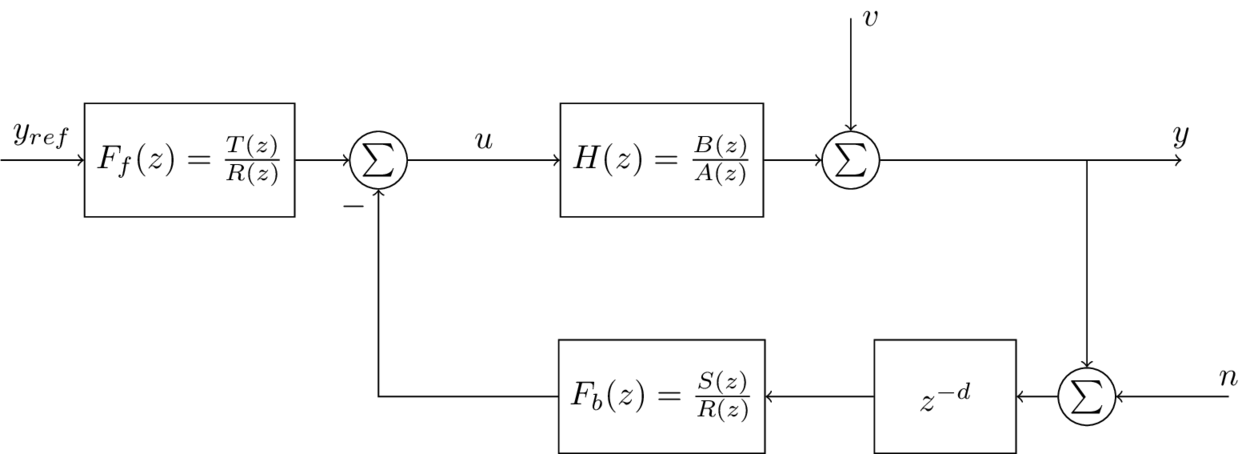
\includegraphics[width=0.8\linewidth]{../../figures/2dof-block-explicit}
\end{center}
\end{frame}

\section{Key concepts}
\label{sec:org724838f}
\begin{frame}[label={sec:orgb8c549e}]{Three key concepts}
\begin{enumerate}
\item Where to place the poles of the closed-loop system.
\item The \emph{sensitivity function} and the \emph{complementary sensitivity function}.
\item How to determine the order of the controller.
\end{enumerate}
\end{frame}

\begin{frame}[label={sec:org1d370d0}]{The closed-loop poles}
Complex poles in the s-plane
\begin{center}
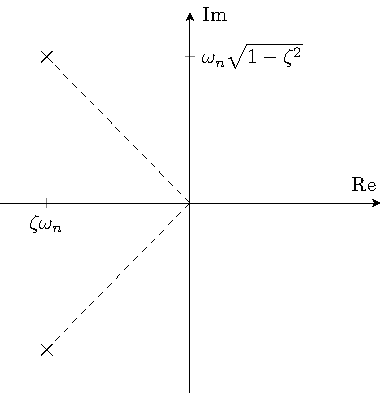
\includegraphics[width=0.45\linewidth]{../../figures/implane-second-order-poles}
\end{center}
\end{frame}

\begin{frame}[label={sec:org190ec43}]{The closed-loop poles}
Given specifications on the velocity and damping of the closed-loop system
\[ t_s \approx \frac{4}{\zeta\omega_n} < 1 s \qquad \zeta \approx \frac{-\ln (\%OS/100)}{\sqrt{\pi^2 + \ln^2(\%OS/100)}}, \quad OS < 10\%  \]
gives
\[ \zeta > 0.59,  \qquad \zeta\omega_n > 4\]

\begin{center}
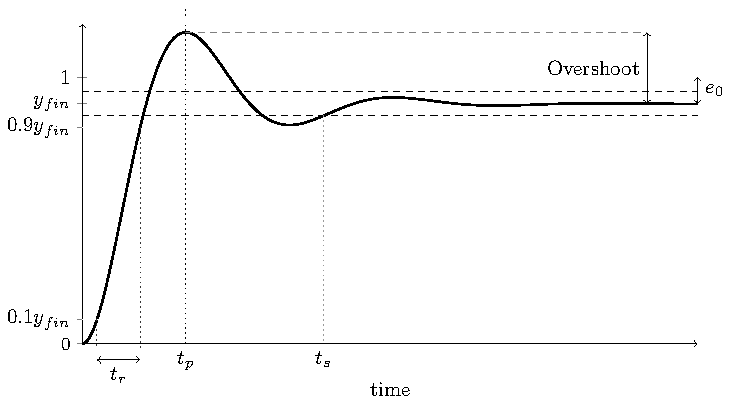
\includegraphics[width=0.6\linewidth]{../../figures/step-response-specifications}
\end{center}
\end{frame}

\begin{frame}[label={sec:org59a4a22}]{Closed-loop poles}
\alert{Activity} Given specifications \(\zeta > 0.59\) and \(\zeta\omega_n > 4\), mark the regions in the s-plane and in the z-plane that corresponds to the specifications. Use sampling period \(h=0.2\).
\begin{center}
\alert{s-plane} \hspace*{0.4\linewidth} \alert{z-plane}\\
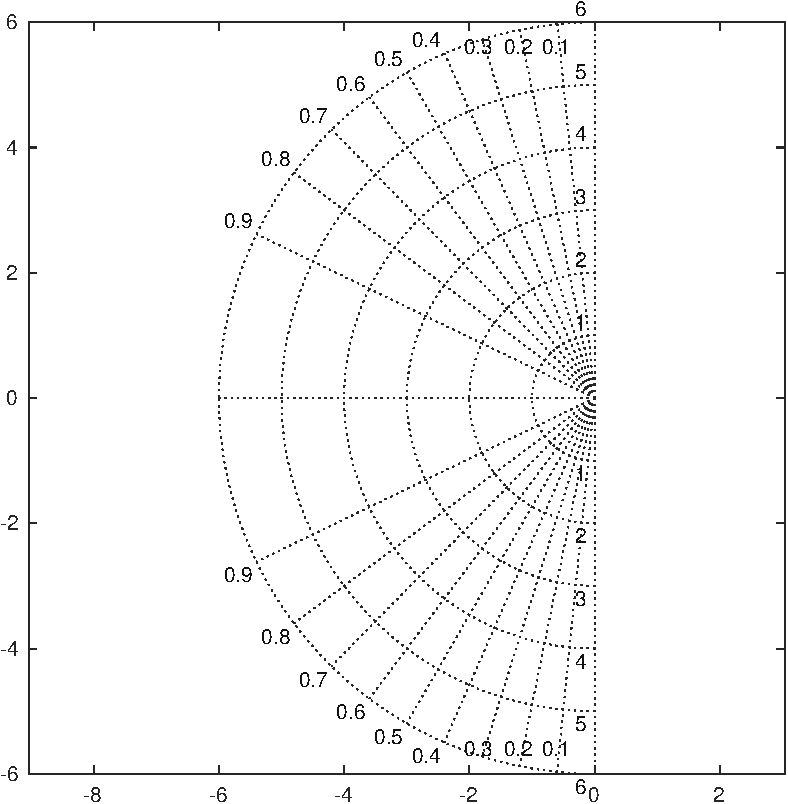
\includegraphics[height=0.61\textheight]{../../figures/sgrid-crop} \hspace*{3mm}
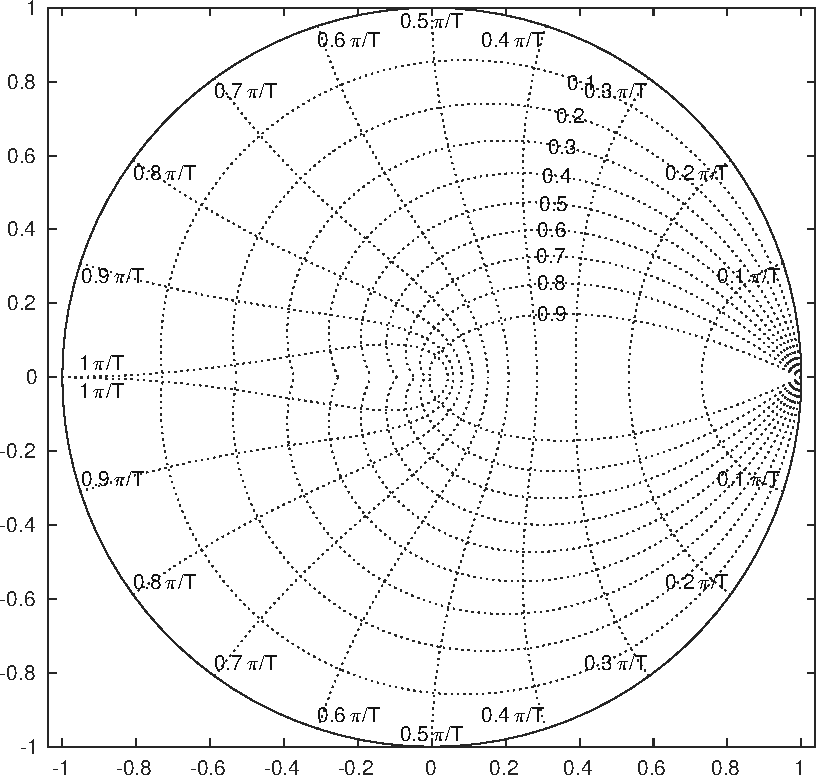
\includegraphics[height=0.6\textheight]{../../figures/zgrid-crop}\\
\end{center}
\end{frame}

\begin{frame}[label={sec:orge304fac}]{The sensitivity and the complementary sensitivity}
\end{frame}
\begin{frame}[label={sec:org9f204b3}]{Two-degree-of-freedom controller}
\begin{center}
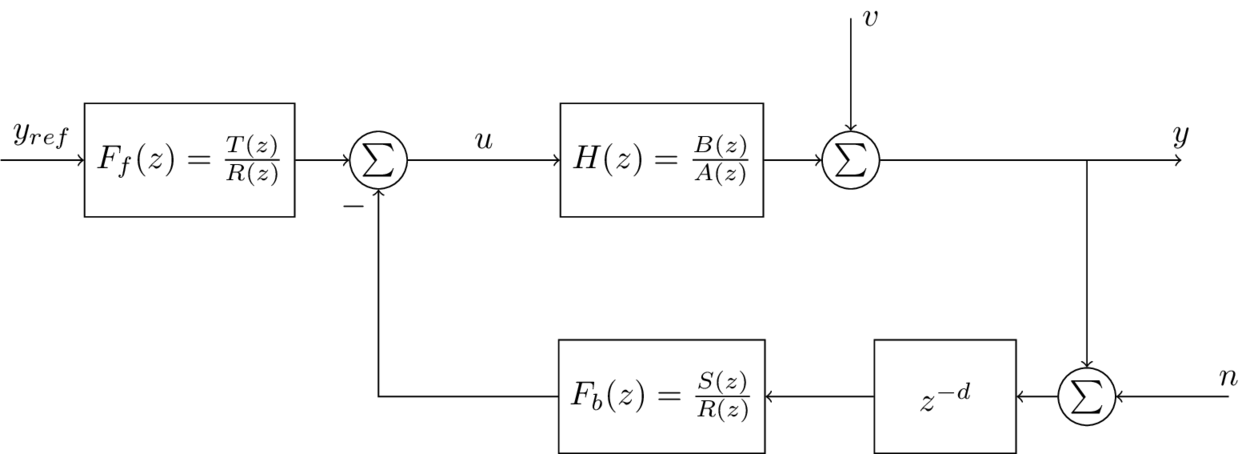
\includegraphics[width=0.8\linewidth]{../../figures/2dof-block-explicit}
\end{center}

\begin{align*}
Y(z) &= G_c(z)Y_{ref}(z) + \overbrace{S_s(z)}^{\text{sens}}V(z) - \overbrace{T_s(z)}^{\text{compl sens}}N(z)\\
     &= \frac{F_f(z)H(z)}{1 + F_b(z)z^{-d}H(z)}U_c(z) + \frac{1}{1 + F_b(z)z^{-d}H(z)}V(z)  - \frac{z^{-d}F_b(z)H(z)}{1 + F_b(z)z^{-d}H(z)}N(z)\\
\end{align*}
\end{frame}

\begin{frame}[label={sec:org803888e}]{Two-degree-of-freedom controller}
\begin{center}
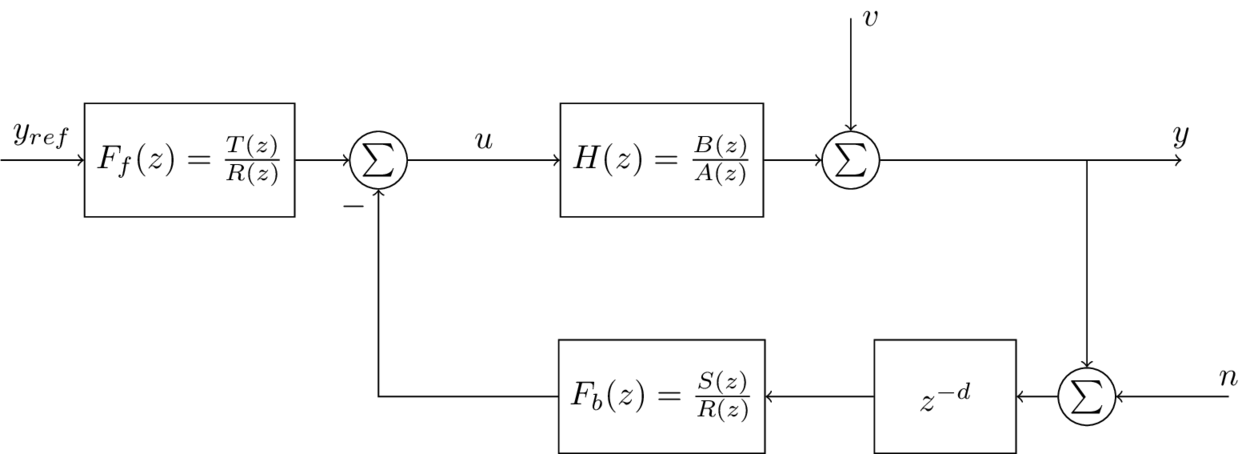
\includegraphics[width=0.7\linewidth]{../../figures/2dof-block-explicit}
\end{center}

\begin{align*}
Y(z)     &= \frac{F_f(z)H(z)}{1 + z^{-d}F_b(z)H(z)}Y_{ref}(z) + \overbrace{\frac{1}{1 + z^{-d}F_b(z)H(z)}}^{S_s(z)}V(z)  - \overbrace{\frac{z^{-d}F_b(z)H(z)}{1 + z^{-d}F_b(z)H(z)}}^{T_s(z)}N(z)\\
\end{align*}

\alert{Evidently} \(S_s(z) + T_s(z) = 1\) \alert{Conclusion:} One must find a balance between disturbance rejection and noise attenuation.
\end{frame}

\begin{frame}[label={sec:org8bea005}]{The sensitivity and the complementary sensitivity}
\begin{columns}
\begin{column}{0.7\columnwidth}
\begin{center}
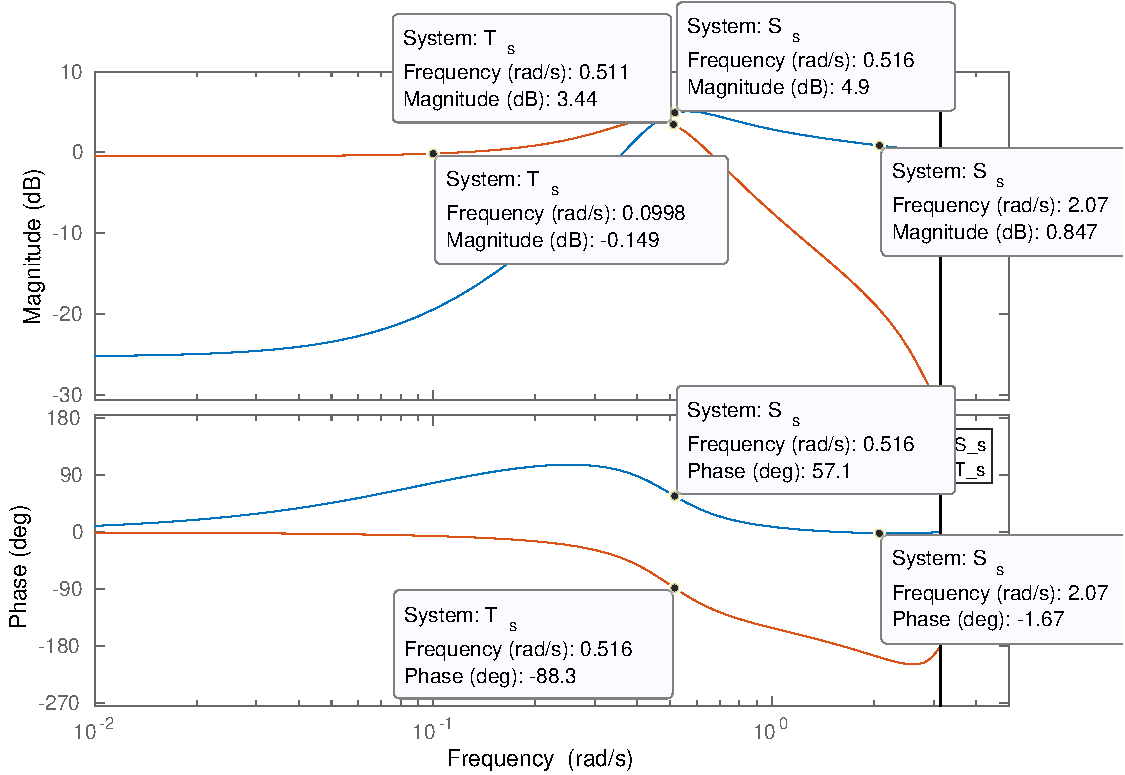
\includegraphics[width=1.05\linewidth]{../matlab/bode-sensitivity-exercise-crop}
\end{center}
\end{column}

\begin{column}{0.3\columnwidth}
\pause

\alert{Activity} Mark in the complex plane the values of \(S_s(z)\) and \(T_s(z)\) for the frequencies 0.511, 0.516 and 2.07 rad/s.  Verify that the vector sum is equal to 1.
\end{column}
\end{columns}
\end{frame}

\begin{frame}[label={sec:orge732f37}]{The sensitivity and the complementary sensitivity}
\pgfmathsetmacro{\Smag}{0.12}
\pgfmathsetmacro{\Sarg}{70}
\pgfmathsetmacro{\Sreal}{\Smag*cos(\Sarg)}
\pgfmathsetmacro{\Sim}{\Smag*sin(\Sarg)}
\pgfmathsetmacro{\Tmag}{0.98}
\pgfmathsetmacro{\Targ}{-6}
\pgfmathsetmacro{\Treal}{\Tmag*cos(\Targ)}
\pgfmathsetmacro{\Tim}{\Tmag*sin(\Targ)}
\alert{Point 1:} \(\omega=0.1\), \(T_s(0.1) = 10^{-0.149/20}\mathrm{e}^{-i6^o} = 0.98\mathrm{e}^{-i6^o} = 0.97 - i0.1\), \(S_s(0.1) = 10^{-18/20}\mathrm{e}^{i70^o} = 0.12\mathrm{e}^{i70^o} = 0.04 + i0.11\)
\begin{center}
  \begin{tikzpicture}[scale=1.6]

    \draw[->] (-2, 0) -- (2, 0) node[below] {Re};
    \draw[->] (0,-2) -- (0,2) node[left] {Im};
    \node[circle, fill, orange, inner sep= 1pt] (Tone) at (\Treal, \Tim) {};
    \draw[thin, ->, orange] (0,0) to (Tone);
    \node[circle, fill, blue!80, inner sep= 1pt] (Sone) at (\Sreal, \Sim) {};
    \draw[thin, ->, blue!80] (0,0) to (Sone);
    \draw (1,0) -- (1,-0.05) node[below] {1};
    \draw (-1,0) -- (-1,-0.05) node[below] {-1};
    \draw (0,1) -- (-0.05,1) node[left] {i};
    \draw (0,-1) -- (-0.05,-1) node[left] {-i};
  \end{tikzpicture}
\end{center}
\end{frame}

\begin{frame}[label={sec:orgb4f03f0}]{The sensitivity and the complementary sensitivity - Solution}
\end{frame}

\begin{frame}[label={sec:org89be80b}]{The sensitivity and the complementary sensitivity - Solution}
\pgfmathsetmacro{\Smag}{0.12}
\pgfmathsetmacro{\Sarg}{70}
\pgfmathsetmacro{\Tmag}{0.98}
\pgfmathsetmacro{\Targ}{-6}
\pgfmathsetmacro{\Treal}{\Tmag*cos(\Targ)}
\pgfmathsetmacro{\Tim}{\Tmag*sin(\Targ)}

\pgfmathsetmacro{\Smagtwo}{0.12}
\pgfmathsetmacro{\Sargtwo}{70}
\pgfmathsetmacro{\Srealtwo}{\Smagtwo*cos(\Sargtwo)}
\pgfmathsetmacro{\Simtwo}{\Smag*sin(\Sarg)}
\pgfmathsetmacro{\Tmagtwo}{0.98}
\pgfmathsetmacro{\Targtwo}{-6}

\begin{center}
  \begin{tikzpicture}[scale=1.6]

    \draw[->] (-2, 0) -- (2, 0) node[below] {Re};
    \draw[->] (0,-2) -- (0,2) node[left] {Im};
    \draw (1,0) -- (1,-0.05) node[below] {1};
    \draw (-1,0) -- (-1,-0.05) node[below] {-1};
    \draw (0,1) -- (-0.05,1) node[left] {i};
    \draw (0,-1) -- (-0.05,-1) node[left] {-i};
 

    \foreach \Tmag/\Targ/\nn in {-0.149/-6/1, 3.44/-88/2, -19/-196/3} {
       \pgfmathsetmacro{\Treal}{pow(10,\Tmag/20)*cos(\Targ)}
       \pgfmathsetmacro{\Tim}{pow(10,\Tmag/20)*sin(\Targ)}
       \node[circle, fill, orange, inner sep= 1pt] (Tone) at (\Treal, \Tim) {};
           \draw[thin, ->, orange] (0,0) to (Tone) node[right] {\tiny \nn};
	   }
    \foreach \Smag/\Sarg/\nn in {-18/78/1, 4.9/57/2, 0.85/-1.67/3} {
       \pgfmathsetmacro{\Sreal}{pow(10,\Smag/20)*cos(\Sarg)}
       \pgfmathsetmacro{\Sim}{pow(10,\Smag/20)*sin(\Sarg)}
       \node[circle, fill, blue!80, inner sep= 1pt] (Sone) at (\Sreal, \Sim) {};
           \draw[thin, ->, blue!80] (0,0) to (Sone) node[right] {\tiny \nn};
	   }

    %\node[circle, fill, blue!80, inner sep= 1pt] (Sone) at (\Sreal, \Sim) {};
    %\draw[thin, ->, blue!80] (0,0) to (Sone);
  \end{tikzpicture}
\end{center}
\end{frame}


\section{RST}
\label{sec:orga1193dc}

\begin{frame}[label={sec:org7845e5f}]{Procedure}
Given plant model \(H(z)=\frac{B(z)}{A(z)}\) and specifications on the desired closed-loop poles \(A_{cl}(z)\)
\begin{enumerate}
\item Find polynomials \(R(z)\) and \(S(z)\) with \(n_R \ge n_S\) such that 
\[ A(z)R(z)z^{d} + B(z)S(z) = A_{cl}(z) \]
\item Factor the closed-loop polynomials as \(A_{cl}(z) = A_c(z)A_o(z)\), where \(n_{A_o} \le n_R\). Choose
\[T(z) = t_0 A_o(z),\] where \(t_0 = \frac{A_c(1)}{B(1)}\).
\end{enumerate}

The control law is then
\[ R(q) u(k) = T(q)u_c(k) - S(q)y(k). \]
The closed-loop response to the command signal is given by
\[ A_c(q)y(k) = t_0 B(q) u_c(k). \]
\end{frame}
\begin{frame}[label={sec:orge8e36f2}]{Determining the order of the controller}
With Diophantine equation 
   \[ A(z)R(z)z^{d} + B(z)S(z) = A_{cl}(z) \qquad (*) \]
and feedback controller
\[F_b(z) = \frac{S(z)}{R(z)} = \frac{s_0z^n + s_1z^{n-1} + \cdots + s_n}{z^n + r_1 z^{n-1} + \cdots + r_n}\]
\alert{How should we choose the order of the controller?} Note:
\begin{itemize}
\item the controller has \(n+n+1 = 2\deg R + 1\) unknown parameters
\item the LHS of \((*)\) has degree \(\deg \big(A(z)R(z)z^d + B(z)S(z)\big) = \deg A + \deg R + d\)
\item The diophantine gives as many (nontrivial) equations as the degree of the polynomials on each side when we set the coefficients equal.

\alert{\(\Rightarrow\;\)Choose \(\deg R\) so that \(2\deg R + 1 = \deg A + \deg R + d\)}
\end{itemize}
\end{frame}


\begin{frame}[label={sec:org4d881a2}]{Determining the order of the controller - Exercise}
With the plant model \[H(z) = \frac{B(z)}{A(z)} = \frac{b}{z + a}\] and \(d=0\) (no delay), what is the appropriate degree of the controller 
\[F_b(z) = \frac{S(z)}{R(z)} = \frac{s_0z^n + s_1z^{n-1} + \cdots + s_n}{z^n + r_1 z^{n-1} + \cdots + r_n}\]
so that all parameters can be determined from the diophantine equation
\[ A(z)R(z) + B(z)S(z) = A_c(z)A_o(z)?\]
\begin{center}
\begin{tabular}{ll}
1. \(n = 0\) & 2. \(n = 1\)\\
3. \(n=2\) & 4. \(n=3\)\\
\end{tabular}
\end{center}
\end{frame}

\begin{frame}[label={sec:orgbaf4096}]{Determining the order of the controller - Exercise - Solution}
With the plant model \[H(z) = \frac{B(z)}{A(z)} = \frac{b}{z + a}\] and \(d=0\) (no delay), what is the appropriate degree of the controller \[F_b(z) = \frac{S(z)}{R(z)} = \frac{s_0z^n + s_1z^{n-1} + \cdots + s_n}{z^n + r_1 z^{n-1} + \cdots + r_n}\]
so that all parameters can be determined from the diophantine equation
\[ A(z)R(z) + B(z)S(z) = A_c(z)A_o(z)?\]
\begin{center}
\begin{tabular}{rr}
1. \(n = 0\) & 2.\\
3. & 4.\\
\end{tabular}
\end{center}
\end{frame}
\end{document}